\documentclass[]{article}
\usepackage{lmodern}
\usepackage{amssymb,amsmath}
\usepackage{ifxetex,ifluatex}
\usepackage{fixltx2e} % provides \textsubscript
\ifnum 0\ifxetex 1\fi\ifluatex 1\fi=0 % if pdftex
  \usepackage[T1]{fontenc}
  \usepackage[utf8]{inputenc}
\else % if luatex or xelatex
  \ifxetex
    \usepackage{mathspec}
  \else
    \usepackage{fontspec}
  \fi
  \defaultfontfeatures{Ligatures=TeX,Scale=MatchLowercase}
\fi
% use upquote if available, for straight quotes in verbatim environments
\IfFileExists{upquote.sty}{\usepackage{upquote}}{}
% use microtype if available
\IfFileExists{microtype.sty}{%
\usepackage{microtype}
\UseMicrotypeSet[protrusion]{basicmath} % disable protrusion for tt fonts
}{}
\usepackage[margin=1in]{geometry}
\usepackage{hyperref}
\hypersetup{unicode=true,
            pdftitle={Personality Data Analysis: Portfolio Project 1},
            pdfauthor={Esben Kran Christensen},
            pdfborder={0 0 0},
            breaklinks=true}
\urlstyle{same}  % don't use monospace font for urls
\usepackage{color}
\usepackage{fancyvrb}
\newcommand{\VerbBar}{|}
\newcommand{\VERB}{\Verb[commandchars=\\\{\}]}
\DefineVerbatimEnvironment{Highlighting}{Verbatim}{commandchars=\\\{\}}
% Add ',fontsize=\small' for more characters per line
\usepackage{framed}
\definecolor{shadecolor}{RGB}{248,248,248}
\newenvironment{Shaded}{\begin{snugshade}}{\end{snugshade}}
\newcommand{\AlertTok}[1]{\textcolor[rgb]{0.94,0.16,0.16}{#1}}
\newcommand{\AnnotationTok}[1]{\textcolor[rgb]{0.56,0.35,0.01}{\textbf{\textit{#1}}}}
\newcommand{\AttributeTok}[1]{\textcolor[rgb]{0.77,0.63,0.00}{#1}}
\newcommand{\BaseNTok}[1]{\textcolor[rgb]{0.00,0.00,0.81}{#1}}
\newcommand{\BuiltInTok}[1]{#1}
\newcommand{\CharTok}[1]{\textcolor[rgb]{0.31,0.60,0.02}{#1}}
\newcommand{\CommentTok}[1]{\textcolor[rgb]{0.56,0.35,0.01}{\textit{#1}}}
\newcommand{\CommentVarTok}[1]{\textcolor[rgb]{0.56,0.35,0.01}{\textbf{\textit{#1}}}}
\newcommand{\ConstantTok}[1]{\textcolor[rgb]{0.00,0.00,0.00}{#1}}
\newcommand{\ControlFlowTok}[1]{\textcolor[rgb]{0.13,0.29,0.53}{\textbf{#1}}}
\newcommand{\DataTypeTok}[1]{\textcolor[rgb]{0.13,0.29,0.53}{#1}}
\newcommand{\DecValTok}[1]{\textcolor[rgb]{0.00,0.00,0.81}{#1}}
\newcommand{\DocumentationTok}[1]{\textcolor[rgb]{0.56,0.35,0.01}{\textbf{\textit{#1}}}}
\newcommand{\ErrorTok}[1]{\textcolor[rgb]{0.64,0.00,0.00}{\textbf{#1}}}
\newcommand{\ExtensionTok}[1]{#1}
\newcommand{\FloatTok}[1]{\textcolor[rgb]{0.00,0.00,0.81}{#1}}
\newcommand{\FunctionTok}[1]{\textcolor[rgb]{0.00,0.00,0.00}{#1}}
\newcommand{\ImportTok}[1]{#1}
\newcommand{\InformationTok}[1]{\textcolor[rgb]{0.56,0.35,0.01}{\textbf{\textit{#1}}}}
\newcommand{\KeywordTok}[1]{\textcolor[rgb]{0.13,0.29,0.53}{\textbf{#1}}}
\newcommand{\NormalTok}[1]{#1}
\newcommand{\OperatorTok}[1]{\textcolor[rgb]{0.81,0.36,0.00}{\textbf{#1}}}
\newcommand{\OtherTok}[1]{\textcolor[rgb]{0.56,0.35,0.01}{#1}}
\newcommand{\PreprocessorTok}[1]{\textcolor[rgb]{0.56,0.35,0.01}{\textit{#1}}}
\newcommand{\RegionMarkerTok}[1]{#1}
\newcommand{\SpecialCharTok}[1]{\textcolor[rgb]{0.00,0.00,0.00}{#1}}
\newcommand{\SpecialStringTok}[1]{\textcolor[rgb]{0.31,0.60,0.02}{#1}}
\newcommand{\StringTok}[1]{\textcolor[rgb]{0.31,0.60,0.02}{#1}}
\newcommand{\VariableTok}[1]{\textcolor[rgb]{0.00,0.00,0.00}{#1}}
\newcommand{\VerbatimStringTok}[1]{\textcolor[rgb]{0.31,0.60,0.02}{#1}}
\newcommand{\WarningTok}[1]{\textcolor[rgb]{0.56,0.35,0.01}{\textbf{\textit{#1}}}}
\usepackage{longtable,booktabs}
\usepackage{graphicx,grffile}
\makeatletter
\def\maxwidth{\ifdim\Gin@nat@width>\linewidth\linewidth\else\Gin@nat@width\fi}
\def\maxheight{\ifdim\Gin@nat@height>\textheight\textheight\else\Gin@nat@height\fi}
\makeatother
% Scale images if necessary, so that they will not overflow the page
% margins by default, and it is still possible to overwrite the defaults
% using explicit options in \includegraphics[width, height, ...]{}
\setkeys{Gin}{width=\maxwidth,height=\maxheight,keepaspectratio}
\IfFileExists{parskip.sty}{%
\usepackage{parskip}
}{% else
\setlength{\parindent}{0pt}
\setlength{\parskip}{6pt plus 2pt minus 1pt}
}
\setlength{\emergencystretch}{3em}  % prevent overfull lines
\providecommand{\tightlist}{%
  \setlength{\itemsep}{0pt}\setlength{\parskip}{0pt}}
\setcounter{secnumdepth}{5}
% Redefines (sub)paragraphs to behave more like sections
\ifx\paragraph\undefined\else
\let\oldparagraph\paragraph
\renewcommand{\paragraph}[1]{\oldparagraph{#1}\mbox{}}
\fi
\ifx\subparagraph\undefined\else
\let\oldsubparagraph\subparagraph
\renewcommand{\subparagraph}[1]{\oldsubparagraph{#1}\mbox{}}
\fi

%%% Use protect on footnotes to avoid problems with footnotes in titles
\let\rmarkdownfootnote\footnote%
\def\footnote{\protect\rmarkdownfootnote}

%%% Change title format to be more compact
\usepackage{titling}

% Create subtitle command for use in maketitle
\providecommand{\subtitle}[1]{
  \posttitle{
    \begin{center}\large#1\end{center}
    }
}

\setlength{\droptitle}{-2em}

  \title{Personality Data Analysis: Portfolio Project 1}
    \pretitle{\vspace{\droptitle}\centering\huge}
  \posttitle{\par}
    \author{Esben Kran Christensen}
    \preauthor{\centering\large\emph}
  \postauthor{\par}
      \predate{\centering\large\emph}
  \postdate{\par}
    \date{9/21/2019}


\begin{document}
\maketitle

{
\setcounter{tocdepth}{2}
\tableofcontents
}
Packages: pacman, bookdown, tidyverse, rticles, RColorBrewer, extrafont, pastec, gridExtra

\hypertarget{abstract}{%
\section{Abstract}\label{abstract}}

This paper investigates the properties of 2019's Cognitive Science Bachelor students at Aarhus University. The students answered and performed 40 questions and actions to accommodate a personality analysis sheet developed by Mikkel Wallentin. In this paper, the data was analyzed using several different data visualization techniques as well as statistical theory.

\hypertarget{introduction}{%
\section{Introduction}\label{introduction}}

The process of analysis performed consists of five different steps:
1. Ocular dominance and lung size.
2. Noise level preferences between females and males.
3. Frequency analysis of held breath times.
4. Frequency analysis of balloon related variables.
5. Correlation between ability to hold breath and shoe size.

\hypertarget{methods}{%
\section{Methods}\label{methods}}

The RStudio IDE and the R programming language is used to perform the analyses of the personality data. Using the aggregated personality data from the 1st semester students, the analyses can be visualized to answer or shed light on the analysis targets outlined above.

\hypertarget{analysis}{%
\section{Analysis}\label{analysis}}

We will start by importing the data into a dataframe in R:

\begin{Shaded}
\begin{Highlighting}[]
\NormalTok{df <-}\StringTok{ }\KeywordTok{read.csv}\NormalTok{(}\StringTok{"NEW_CogSciPersonalityTest2019.csv"}\NormalTok{)}
\end{Highlighting}
\end{Shaded}

\hypertarget{ocular-dominance-and-lung-size}{%
\subsection{Ocular dominance and lung size}\label{ocular-dominance-and-lung-size}}

Who can hold their breath longer on average, those with right or left ocular dominance? By using the ggplot2 package in RStudio and performing a summary analysis with the dplyr::summarise function, the differences in ability to hold their breath between 1st semester students with right ocular dominance and left ocular dominance can be analyzed.

We'll start by removing the rows where the ocular dominance is equals to ``Both'' as it is irrelevant to analyzing differences between left and right ocular dominance and the probability of not having any ocular dominance (``Both'') is below 1\% in healthy adults (see Eser et al. 2008).

\begin{Shaded}
\begin{Highlighting}[]
\NormalTok{F_both_od <-}\StringTok{ }\NormalTok{df[df}\OperatorTok{$}\NormalTok{ocular_dom }\OperatorTok{!=}\StringTok{ "Both"}\NormalTok{, ]}
\end{Highlighting}
\end{Shaded}

Secondly, we'll plot the mean breath\_hold according to the ocular dominance to see how they match up visually:

\begin{Shaded}
\begin{Highlighting}[]
\KeywordTok{ggplot}\NormalTok{(F_both_od, }\KeywordTok{aes}\NormalTok{(}\DataTypeTok{x =}\NormalTok{ F_both_od}\OperatorTok{$}\NormalTok{ocular_dom, }\DataTypeTok{y =}\NormalTok{ F_both_od}\OperatorTok{$}\NormalTok{breath_hold, }\DataTypeTok{fill =}\NormalTok{ F_both_od}\OperatorTok{$}\NormalTok{ocular_dom)) }\OperatorTok{+}\StringTok{ }
\StringTok{    }\KeywordTok{geom_boxplot}\NormalTok{() }\OperatorTok{+}\StringTok{ }\KeywordTok{geom_point}\NormalTok{(}\DataTypeTok{stat =} \StringTok{"summary"}\NormalTok{, }\DataTypeTok{fun.y =}\NormalTok{ mean, ) }\OperatorTok{+}\StringTok{ }\KeywordTok{geom_errorbar}\NormalTok{(}\DataTypeTok{show.legend =}\NormalTok{ F, }
    \DataTypeTok{stat =} \StringTok{"summary"}\NormalTok{, }\DataTypeTok{fun.data =}\NormalTok{ mean_se, }\DataTypeTok{width =} \FloatTok{0.1}\NormalTok{) }\OperatorTok{+}\StringTok{ }\KeywordTok{labs}\NormalTok{(}\DataTypeTok{x =} \StringTok{"Ocular dominance"}\NormalTok{, }
    \DataTypeTok{y =} \StringTok{"Breath held time"}\NormalTok{) }\OperatorTok{+}\StringTok{ }\KeywordTok{theme_minimal}\NormalTok{()}
\end{Highlighting}
\end{Shaded}

\begin{figure}
\centering
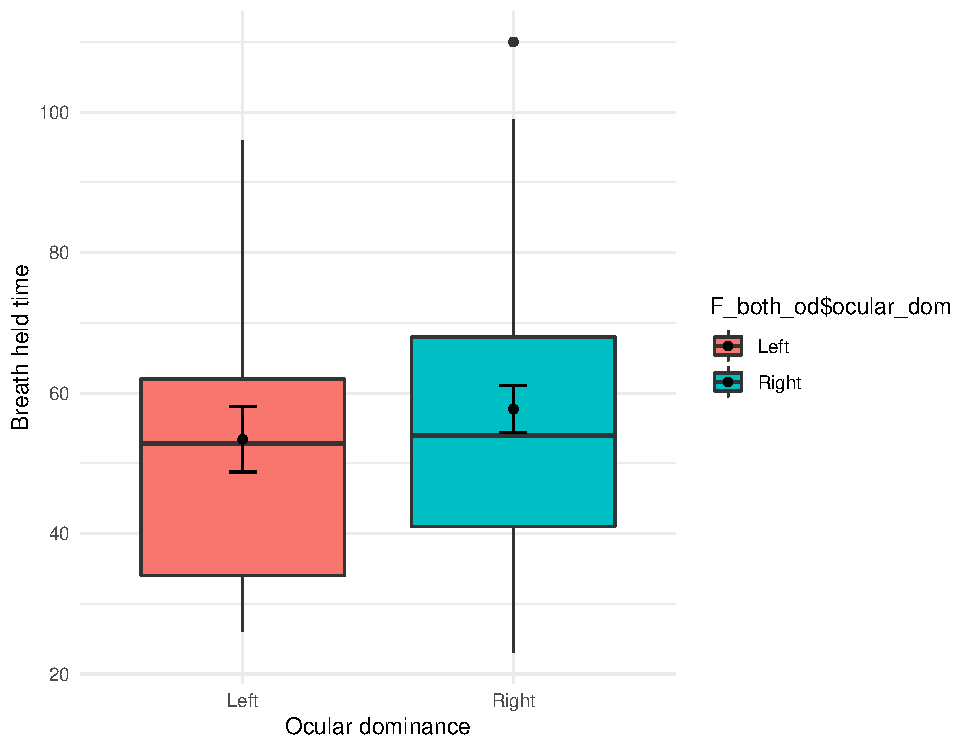
\includegraphics{Personality-Data-Analysis-Portfolio-1_files/figure-latex/unnamed-chunk-3-1.pdf}
\caption{\label{fig:unnamed-chunk-3}Plotting breath\_hold by ocular\_dom}
\end{figure}

The dot with the black error bars is the mean with mean standard error error bars appended.

By looking at the boxplot and seeing that the SEM error bars overlap, we can conclude from a simplification of \href{https://www.graphpad.com/support/faq/spanwhat-you-can-conclude-when-two-error-bars-overlap-or-dontspan/}{Cumming's (2007)} rules on statistical significance that the P-value is \emph{much} greater than 0.05 which means the difference is not statistically significant.

We can therefore conclude that there is no large difference between groups of differing ocular dominance and the ability to hold their breath.

\hypertarget{noise-level-preferences-between-females-and-males}{%
\subsection{Noise level preferences between females and males}\label{noise-level-preferences-between-females-and-males}}

Who likes silence versus noise the best? Males or females? By using the same process as in the previous step, we can perform an analysis of the gender dissonance in noise preferences. But first, we will plot the data to find out if there are any outliers

\begin{Shaded}
\begin{Highlighting}[]
\KeywordTok{ggplot}\NormalTok{(df) }\OperatorTok{+}\StringTok{ }\KeywordTok{geom_histogram}\NormalTok{(}\DataTypeTok{binwidth =} \DecValTok{4}\NormalTok{, }\KeywordTok{aes}\NormalTok{(}\DataTypeTok{x =}\NormalTok{ df}\OperatorTok{$}\NormalTok{sound_level_pref, }\DataTypeTok{y =}\NormalTok{ ..count.., }
    \DataTypeTok{fill =}\NormalTok{ df}\OperatorTok{$}\NormalTok{gender), }\DataTypeTok{colour =} \StringTok{"black"}\NormalTok{) }\OperatorTok{+}\StringTok{ }\KeywordTok{theme_minimal}\NormalTok{() }\OperatorTok{+}\StringTok{ }\KeywordTok{labs}\NormalTok{(}\DataTypeTok{x =} \StringTok{"Sound level preference"}\NormalTok{, }
    \DataTypeTok{y =} \StringTok{"Count"}\NormalTok{)}
\end{Highlighting}
\end{Shaded}

\begin{figure}
\centering
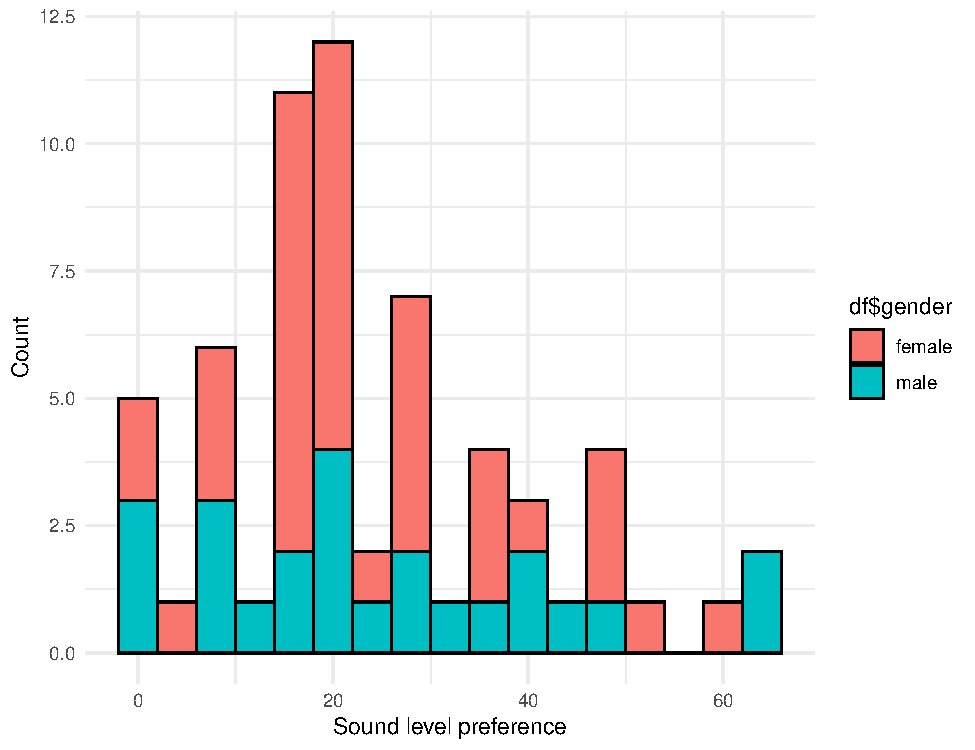
\includegraphics{Personality-Data-Analysis-Portfolio-1_files/figure-latex/unnamed-chunk-4-1.pdf}
\caption{\label{fig:unnamed-chunk-4}Histogram of sound level preference}
\end{figure}

As there are no significant outliers, we will commence the analysis with the dplyr::summarise\_each function:

\begin{Shaded}
\begin{Highlighting}[]
\NormalTok{df }\OperatorTok\StringTok{ }\KeywordTok{group_by}\NormalTok{(gender) }\OperatorTok\StringTok{ }\KeywordTok{summarise_each}\NormalTok{(}\KeywordTok{funs}\NormalTok{(mean, sd), }\DataTypeTok{noise =}\NormalTok{ sound_level_pref, }
    \DataTypeTok{noise =}\NormalTok{ sound_level_pref)}
\end{Highlighting}
\end{Shaded}

\begin{verbatim}
> # A tibble: 2 x 3
>   gender noise_mean noise_sd
>   <fct>       <dbl>    <dbl>
> 1 female       24.3     14.6
> 2 male         25.6     18.5
\end{verbatim}

Through a purely numeric argumentation, we can see that the gender difference is completely negligible through mean and standard deviance differences between males and females. By trying to plot the gender differences in a bar plot with an error bars layer in ggplot2, we can see that no real differences are visible except larger center aggregation of values in female data (which could be seen as quite interesting from cultural bias perspective).

\begin{Shaded}
\begin{Highlighting}[]
\KeywordTok{ggplot}\NormalTok{(df, }\KeywordTok{aes}\NormalTok{(}\DataTypeTok{x =}\NormalTok{ gender, }\DataTypeTok{y =}\NormalTok{ sound_level_pref, }\DataTypeTok{fill =}\NormalTok{ gender)) }\OperatorTok{+}\StringTok{ }\KeywordTok{geom_boxplot}\NormalTok{() }\OperatorTok{+}\StringTok{ }
\StringTok{    }\KeywordTok{geom_errorbar}\NormalTok{(}\DataTypeTok{stat =} \StringTok{"summary"}\NormalTok{, }\DataTypeTok{fun.data =}\NormalTok{ mean_se, }\DataTypeTok{width =} \FloatTok{0.1}\NormalTok{) }\OperatorTok{+}\StringTok{ }\KeywordTok{geom_point}\NormalTok{(}\DataTypeTok{stat =} \StringTok{"summary"}\NormalTok{, }
    \DataTypeTok{fun.y =}\NormalTok{ mean, ) }\OperatorTok{+}\StringTok{ }\KeywordTok{labs}\NormalTok{(}\DataTypeTok{x =} \StringTok{"Gender"}\NormalTok{, }\DataTypeTok{y =} \StringTok{"Noise level preference"}\NormalTok{) }\OperatorTok{+}\StringTok{ }\KeywordTok{theme_minimal}\NormalTok{()}
\end{Highlighting}
\end{Shaded}

\begin{figure}
\centering
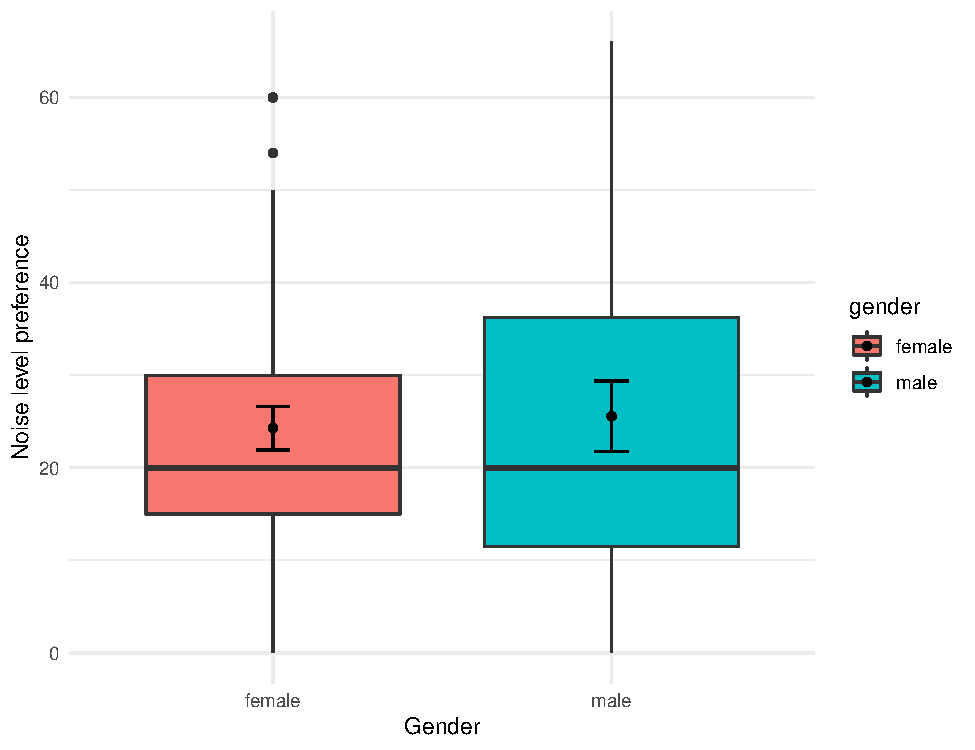
\includegraphics{Personality-Data-Analysis-Portfolio-1_files/figure-latex/unnamed-chunk-6-1.pdf}
\caption{\label{fig:unnamed-chunk-6}Noise level preference by gender}
\end{figure}

The visual explanation is the same as in the previous analysis process step: As the SEM error bars overlap, we can conclude from a simplification of \href{https://www.graphpad.com/support/faq/spanwhat-you-can-conclude-when-two-error-bars-overlap-or-dontspan/}{Cumming's (2007)} rules on statistical significance that the P-value is \emph{much} greather than 0.05 which means the difference is not statistically significant.

\hypertarget{frequency-analysis-of-held-breath-times}{%
\subsection{Frequency analysis of held breath times}\label{frequency-analysis-of-held-breath-times}}

Is the breath\_hold data normally distributed? With visual and numeric support, an analysis to determine this is executed using ggplot2 plotting powers. We will define this plotting as a function to ease comprehension and for later usage.

\begin{Shaded}
\begin{Highlighting}[]
\NormalTok{e_freq_distribution <-}\StringTok{ }\ControlFlowTok{function}\NormalTok{(dataframe, x, title) \{}
    \KeywordTok{ggplot}\NormalTok{(dataframe, }\KeywordTok{aes}\NormalTok{(}\DataTypeTok{x =}\NormalTok{ x)) }\OperatorTok{+}\StringTok{ }\KeywordTok{geom_histogram}\NormalTok{(}\DataTypeTok{binwidth =} \DecValTok{2}\NormalTok{, }\DataTypeTok{colour =} \StringTok{"black"}\NormalTok{, }
        \KeywordTok{aes}\NormalTok{(}\DataTypeTok{y =}\NormalTok{ ..density.., }\DataTypeTok{fill =}\NormalTok{ ..count..)) }\OperatorTok{+}\StringTok{ }\KeywordTok{scale_fill_gradient}\NormalTok{(}\StringTok{"Count"}\NormalTok{) }\OperatorTok{+}\StringTok{ }
\StringTok{        }\KeywordTok{stat_function}\NormalTok{(}\DataTypeTok{fun =}\NormalTok{ dnorm, }\DataTypeTok{color =} \StringTok{"orangered2"}\NormalTok{, }\DataTypeTok{size =} \DecValTok{1}\NormalTok{, }\DataTypeTok{args =} \KeywordTok{list}\NormalTok{(}\DataTypeTok{mean =} \KeywordTok{mean}\NormalTok{(x), }
            \DataTypeTok{sd =} \KeywordTok{sd}\NormalTok{(x))) }\OperatorTok{+}\StringTok{ }\KeywordTok{labs}\NormalTok{(}\DataTypeTok{title =}\NormalTok{ title, }\DataTypeTok{subtitle =} \StringTok{"Using dnorm() to create normal distribution line (orange)"}\NormalTok{, }
        \DataTypeTok{x =} \StringTok{"Time"}\NormalTok{, }\DataTypeTok{y =} \StringTok{"Density"}\NormalTok{) }\OperatorTok{+}\StringTok{ }\KeywordTok{theme_minimal}\NormalTok{()}
\NormalTok{\}}
\end{Highlighting}
\end{Shaded}

And using the custom function with the variable inputs as well as a qq-plot:

\begin{Shaded}
\begin{Highlighting}[]
\NormalTok{ggplot1 <-}\StringTok{ }\KeywordTok{e_freq_distribution}\NormalTok{(df, df}\OperatorTok{$}\NormalTok{breath_hold, }\StringTok{"Held breath time frequency density"}\NormalTok{)}
\NormalTok{ggplot2 <-}\StringTok{ }\KeywordTok{ggplot}\NormalTok{(df, }\KeywordTok{aes}\NormalTok{(}\DataTypeTok{sample =}\NormalTok{ df}\OperatorTok{$}\NormalTok{breath_hold)) }\OperatorTok{+}\StringTok{ }\KeywordTok{stat_qq}\NormalTok{() }\OperatorTok{+}\StringTok{ }\KeywordTok{stat_qq_line}\NormalTok{() }\OperatorTok{+}\StringTok{ }
\StringTok{    }\KeywordTok{labs}\NormalTok{(}\DataTypeTok{y =} \StringTok{"Breath hold"}\NormalTok{, }\DataTypeTok{title =} \StringTok{"QQ-plot of breath hold times"}\NormalTok{) }\OperatorTok{+}\StringTok{ }\KeywordTok{theme_minimal}\NormalTok{()}
\NormalTok{ggplot3 <-}\StringTok{ }\KeywordTok{ggplot}\NormalTok{(df, }\KeywordTok{aes}\NormalTok{(}\DataTypeTok{x =}\NormalTok{ df}\OperatorTok{$}\NormalTok{breath_hold, }\DataTypeTok{y =}\NormalTok{ ..density.., }\DataTypeTok{fill =}\NormalTok{ gender)) }\OperatorTok{+}\StringTok{ }
\StringTok{    }\KeywordTok{geom_density}\NormalTok{(}\DataTypeTok{alpha =} \FloatTok{0.7}\NormalTok{) }\OperatorTok{+}\StringTok{ }\KeywordTok{theme_minimal}\NormalTok{() }\OperatorTok{+}\StringTok{ }\KeywordTok{labs}\NormalTok{(}\DataTypeTok{x =} \StringTok{"Breath hold"}\NormalTok{)}

\KeywordTok{grid.arrange}\NormalTok{(ggplot1, ggplot2, ggplot3, }\DataTypeTok{nrow =} \DecValTok{2}\NormalTok{, }\DataTypeTok{ncol =} \DecValTok{2}\NormalTok{)}
\end{Highlighting}
\end{Shaded}

\begin{figure}
\centering
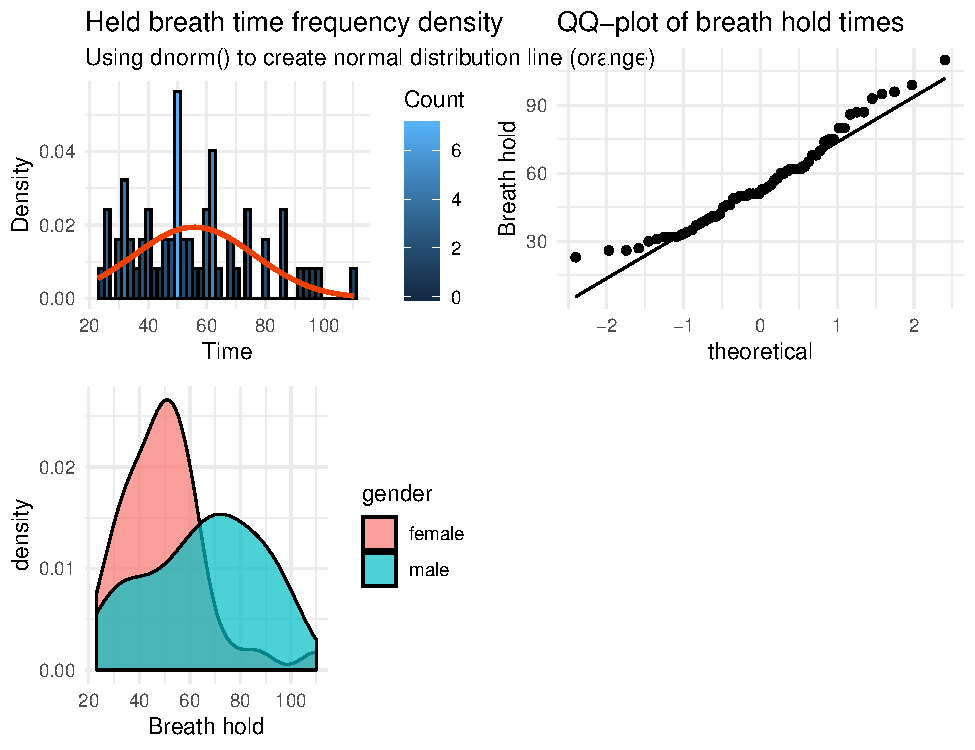
\includegraphics{Personality-Data-Analysis-Portfolio-1_files/figure-latex/unnamed-chunk-8-1.pdf}
\caption{\label{fig:unnamed-chunk-8}Plotting a frequency distribution, density plot and QQ-plot beside each other}
\end{figure}

With the quantile-quantile plot (QQ-plot), we can see how much the breath\_hold data (y axis) resembles a theoretically perfect normal distribution (x axis) quantile for quantile. The linear function indicates the perfect normal distribution. We can see that the breath\_hold data correlates roughly to this linear function which indicates that the data \emph{might} follow a normal distribution though it is doubtful as it still deviates quite a lot.

Therefore, to be completely sure, we can test it using the Shapiro-Wilk test that returns the p-value for the probability that the data rejects the null-hypothesis that it follows a normal distribution:

With the Shapiro-Wilk test output of 0.035 (normtest.p = 3.5\%), we can see that we will have to reject the null-hypothesis that the breath\_hold data follows a normal distribution. But let's keep this thought and hypothesize that the reason for the failed Shapiro-Wilk normality test is because the data is binomial because of the difference between female and male breath\_hold times (see figure 3.4):

\begin{Shaded}
\begin{Highlighting}[]
\KeywordTok{stat.desc}\NormalTok{(df[df}\OperatorTok{$}\NormalTok{gender }\OperatorTok{==}\StringTok{ "male"}\NormalTok{, }\KeywordTok{c}\NormalTok{(}\StringTok{"breath_hold"}\NormalTok{)], df}\OperatorTok{$}\NormalTok{breath_hold, }\DataTypeTok{basic =}\NormalTok{ F, }
    \DataTypeTok{norm =}\NormalTok{ T)}
\end{Highlighting}
\end{Shaded}

\begin{verbatim}
>   skewness   skew.2SE   kurtosis   kurt.2SE normtest.W normtest.p 
> -0.2381634 -0.2521524 -1.2139052 -0.6613290  0.9450407  0.2110520
\end{verbatim}

\begin{Shaded}
\begin{Highlighting}[]
\KeywordTok{stat.desc}\NormalTok{(df[df}\OperatorTok{$}\NormalTok{gender }\OperatorTok{==}\StringTok{ "female"}\NormalTok{, }\KeywordTok{c}\NormalTok{(}\StringTok{"breath_hold"}\NormalTok{)], df}\OperatorTok{$}\NormalTok{breath_hold, }\DataTypeTok{basic =}\NormalTok{ F, }
    \DataTypeTok{norm =}\NormalTok{ T)[]}
\end{Highlighting}
\end{Shaded}

\begin{verbatim}
>    skewness    skew.2SE    kurtosis    kurt.2SE  normtest.W  normtest.p 
> 1.211480885 1.582317996 2.563814041 1.709892516 0.912328039 0.005788547
\end{verbatim}

Using this data, we might be able to conclude that the male data for breath\_hold follows a normal distribution (\texttt{normtest.p} \textgreater{} 0.05) while the female data definitely does not (\texttt{normtest.p} \textless{} 0.05). A probable reason for these differences and results might be the sample size. But as we are analyzing this specific sample's distribution, the conclusions are correct in relation to this exact population.

\hypertarget{frequency-analysis-of-balloon-related-variables}{%
\subsection{Frequency analysis of balloon related variables}\label{frequency-analysis-of-balloon-related-variables}}

Is the balloon and balloon\_balance data normally distributed? With visual and numeric support, an analysis to determine this is performed using ggplot2 plotting capabilities and statistics analysis.

\begin{Shaded}
\begin{Highlighting}[]
\KeywordTok{e_freq_distribution}\NormalTok{(df, df}\OperatorTok{$}\NormalTok{balloon, }\StringTok{"Balloon blow-up time histogram"}\NormalTok{)}
\end{Highlighting}
\end{Shaded}

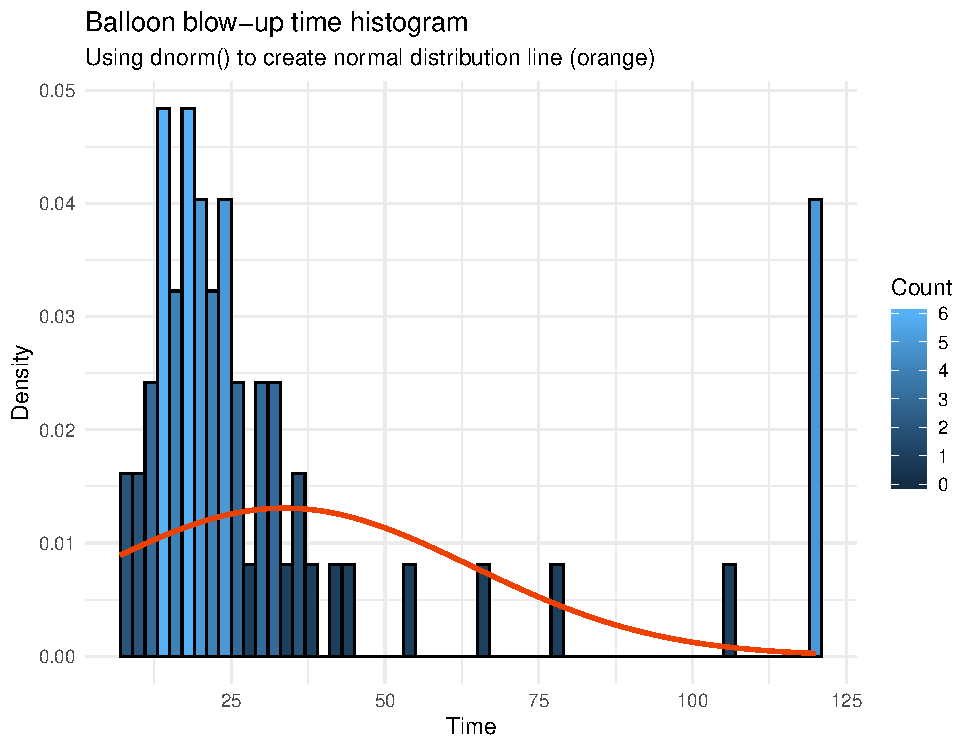
\includegraphics{Personality-Data-Analysis-Portfolio-1_files/figure-latex/unnamed-chunk-10-1.pdf}
We can see that the normal distribution's kurtosis and skew is drastically affected by the outlier in the higher end of the scale. We will try to identify numerically that this outlier has a large effect on the data:

\begin{Shaded}
\begin{Highlighting}[]
\NormalTok{getmode <-}\StringTok{ }\ControlFlowTok{function}\NormalTok{(v) \{}
\NormalTok{    uniqv <-}\StringTok{ }\KeywordTok{unique}\NormalTok{(v)}
    \KeywordTok{return}\NormalTok{(uniqv[}\KeywordTok{which.max}\NormalTok{(}\KeywordTok{tabulate}\NormalTok{(}\KeywordTok{match}\NormalTok{(v, uniqv)))])}
\NormalTok{\}}

\NormalTok{mode <-}\StringTok{ }\KeywordTok{getmode}\NormalTok{(df}\OperatorTok{$}\NormalTok{balloon)}
\KeywordTok{names}\NormalTok{(mode) <-}\StringTok{ }\KeywordTok{c}\NormalTok{(}\StringTok{"mode"}\NormalTok{)}
\KeywordTok{print}\NormalTok{(mode)}
\end{Highlighting}
\end{Shaded}

\begin{verbatim}
> mode 
>   15
\end{verbatim}

\begin{Shaded}
\begin{Highlighting}[]
\KeywordTok{round}\NormalTok{(}\KeywordTok{stat.desc}\NormalTok{(df}\OperatorTok{$}\NormalTok{balloon, }\DataTypeTok{basic =}\NormalTok{ F, }\DataTypeTok{norm =}\NormalTok{ T), }\DataTypeTok{digits =} \DecValTok{3}\NormalTok{)}
\end{Highlighting}
\end{Shaded}

\begin{verbatim}
>       median         mean      SE.mean CI.mean.0.95          var 
>       22.500       33.677        3.874        7.746      930.403 
>      std.dev     coef.var     skewness     skew.2SE     kurtosis 
>       30.503        0.906        2.010        3.306        2.852 
>     kurt.2SE   normtest.W   normtest.p 
>        2.379        0.660        0.000
\end{verbatim}

Using the summarise function, we can see that the mean, mode and median are significantly different, signifying that there's an outlier that has a strong influence on especially the mean (33.7 s) compared to the median and the mode (22.5 s and 15 s respectively). Additionally, the stat.desc shows us that the normal distribution has a major skew.2SE (2 standard error) of 3.306 (is 1 for standard normal distribution) which shows us that the data includes values that skews the data (outlier).

We will try to exclude the outlier by excluding any values deviating by 2.58 standard deviations from the mean and re-plotting the histogram. By using the value of 2.58 we practically exclude results that are below a 1\% chance of existing in normally distributed populations - a z-score under 2.58 = 99.012\% probability of being under the distribution curve.

\begin{Shaded}
\begin{Highlighting}[]
\NormalTok{sd_b <-}\StringTok{ }\KeywordTok{sd}\NormalTok{(df}\OperatorTok{$}\NormalTok{balloon)}
\NormalTok{b_258sd_df <-}\StringTok{ }\NormalTok{df[df}\OperatorTok{$}\NormalTok{balloon }\OperatorTok{<}\StringTok{ }\KeywordTok{mean}\NormalTok{(df}\OperatorTok{$}\NormalTok{balloon) }\OperatorTok{+}\StringTok{ }\FloatTok{2.58} \OperatorTok{*}\StringTok{ }\NormalTok{sd_b }\OperatorTok{&}\StringTok{ }\NormalTok{df}\OperatorTok{$}\NormalTok{balloon }\OperatorTok{>}\StringTok{ }
\StringTok{    }\KeywordTok{mean}\NormalTok{(df}\OperatorTok{$}\NormalTok{balloon) }\OperatorTok{-}\StringTok{ }\FloatTok{2.58} \OperatorTok{*}\StringTok{ }\NormalTok{sd_b, ]}
\KeywordTok{e_freq_distribution}\NormalTok{(b_258sd_df, b_258sd_df}\OperatorTok{$}\NormalTok{balloon, }\StringTok{"Balloon blow-up time histogram without outlier"}\NormalTok{)}
\end{Highlighting}
\end{Shaded}

\begin{figure}
\centering
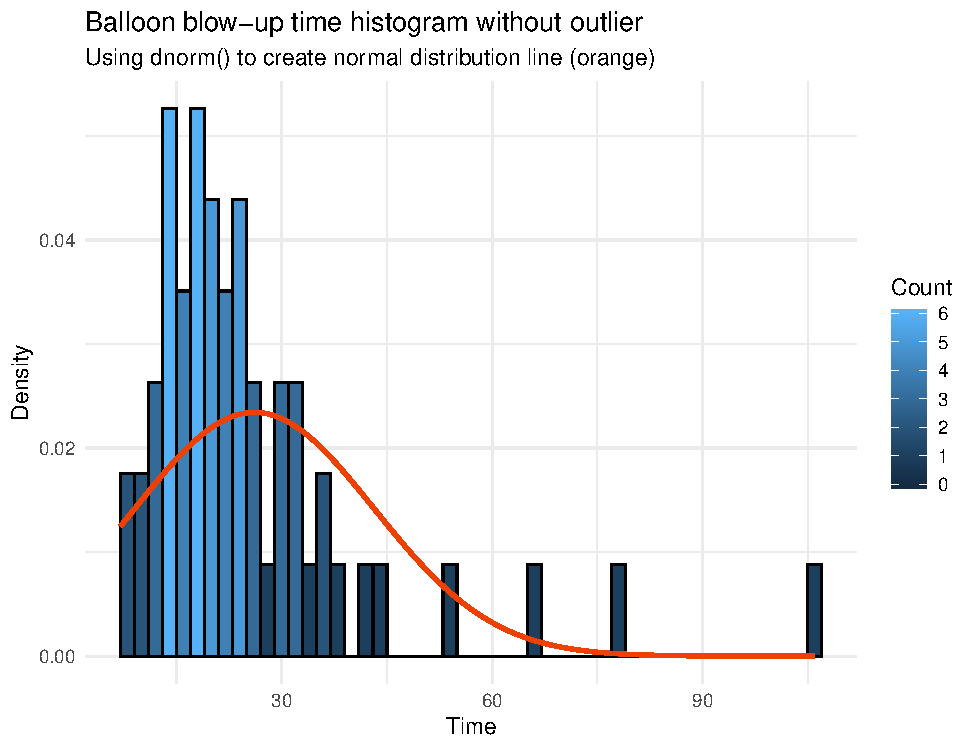
\includegraphics{Personality-Data-Analysis-Portfolio-1_files/figure-latex/unnamed-chunk-12-1.pdf}
\caption{\label{fig:unnamed-chunk-12}Removing outliers (-2.58 \textless{} z \textless{} 2.58) and re-plotting the histogram}
\end{figure}

Here we can see how the distribution fits a normal distribution better visually but would still have a skew if plotted without dnorm() function. We can do a numeric summary using the stat.desc once more to see if we have more normally distributed data after removing the outlier:

\begin{Shaded}
\begin{Highlighting}[]
\KeywordTok{round}\NormalTok{(}\KeywordTok{stat.desc}\NormalTok{(b_258sd_df}\OperatorTok{$}\NormalTok{balloon, }\DataTypeTok{basic =}\NormalTok{ F, }\DataTypeTok{norm =}\NormalTok{ T), }\DataTypeTok{digits =} \DecValTok{3}\NormalTok{)}
\end{Highlighting}
\end{Shaded}

\begin{verbatim}
>       median         mean      SE.mean CI.mean.0.95          var 
>       22.000       26.105        2.255        4.517      289.793 
>      std.dev     coef.var     skewness     skew.2SE     kurtosis 
>       17.023        0.652        2.536        4.009        7.919 
>     kurt.2SE   normtest.W   normtest.p 
>        6.354        0.740        0.000
\end{verbatim}

The skew has increased unexpectedly. The reason for this is probably the fact that the previous skew was caused by the data having a lower boundary because the data is time-based and starts from 0. As there are no possible values below zero, the skew is therefore expected and we cannot say that the data is normally distributed (normtest.p \textless{} 0.05) even though it might look that way on the graph. Additionally, it is a positive skew so this could have been analyzed from the first skewness calculation.

\hypertarget{correlation-between-ability-to-hold-breath-and-shoe-size}{%
\subsection{Correlation between ability to hold breath and shoe size}\label{correlation-between-ability-to-hold-breath-and-shoe-size}}

Shoe size could tell us something about general body size, which could also be connected to one's ability to hold one's breath. In other words, we predict that there is a positive relation between shoe size and how long time CogSci students can hold their breath.
By plotting the two sets of data against each other on a scatter plot and analyzing differences between males and females, we can see how shoe size affects the ability to hold one's breath.

\begin{Shaded}
\begin{Highlighting}[]
\KeywordTok{p_load}\NormalTok{(gridExtra)}

\NormalTok{plot1 <-}\StringTok{ }\KeywordTok{ggplot}\NormalTok{(df, }\KeywordTok{aes}\NormalTok{(}\DataTypeTok{x =}\NormalTok{ df}\OperatorTok{$}\NormalTok{shoesize, }\DataTypeTok{y =}\NormalTok{ df}\OperatorTok{$}\NormalTok{breath_hold)) }\OperatorTok{+}\StringTok{ }\KeywordTok{geom_point}\NormalTok{(}\DataTypeTok{show.legend =}\NormalTok{ F, }
    \KeywordTok{aes}\NormalTok{(}\DataTypeTok{color =}\NormalTok{ df}\OperatorTok{$}\NormalTok{gender)) }\OperatorTok{+}\StringTok{ }\KeywordTok{geom_smooth}\NormalTok{(}\DataTypeTok{show.legend =}\NormalTok{ F, }\DataTypeTok{formula =}\NormalTok{ y }\OperatorTok{~}\StringTok{ }\NormalTok{x, }
    \DataTypeTok{method =} \StringTok{"lm"}\NormalTok{, }\DataTypeTok{color =} \StringTok{"#2c3e50"}\NormalTok{) }\OperatorTok{+}\StringTok{ }\KeywordTok{labs}\NormalTok{(}\DataTypeTok{title =} \StringTok{"1: Correlation between shoe size}\CharTok{\textbackslash{}n}\StringTok{and breath hold time"}\NormalTok{, }
    \DataTypeTok{subtitle =} \StringTok{"Blue = male, red = female"}\NormalTok{, }\DataTypeTok{x =} \StringTok{"Shoe Size"}\NormalTok{, }\DataTypeTok{y =} \StringTok{"Breath hold time"}\NormalTok{) }\OperatorTok{+}\StringTok{ }
\StringTok{    }\KeywordTok{theme_grey}\NormalTok{()}

\NormalTok{plot2 <-}\StringTok{ }\KeywordTok{ggplot}\NormalTok{(df, }\KeywordTok{aes}\NormalTok{(}\DataTypeTok{x =}\NormalTok{ df}\OperatorTok{$}\NormalTok{shoesize, }\DataTypeTok{y =}\NormalTok{ df}\OperatorTok{$}\NormalTok{breath_hold, }\DataTypeTok{color =}\NormalTok{ df}\OperatorTok{$}\NormalTok{gender)) }\OperatorTok{+}\StringTok{ }
\StringTok{    }\KeywordTok{geom_point}\NormalTok{(}\DataTypeTok{show.legend =}\NormalTok{ F) }\OperatorTok{+}\StringTok{ }\KeywordTok{geom_smooth}\NormalTok{(}\DataTypeTok{show.legend =}\NormalTok{ F, }\DataTypeTok{formula =}\NormalTok{ y }\OperatorTok{~}\StringTok{ }
\StringTok{    }\NormalTok{x, }\DataTypeTok{method =} \StringTok{"lm"}\NormalTok{) }\OperatorTok{+}\StringTok{ }\KeywordTok{labs}\NormalTok{(}\DataTypeTok{title =} \StringTok{"2: Gender difference"}\NormalTok{, }\DataTypeTok{subtitle =} \StringTok{"Blue = male, red = female"}\NormalTok{, }
    \DataTypeTok{x =} \StringTok{"Shoe Size"}\NormalTok{, }\DataTypeTok{y =} \StringTok{"Breath hold time"}\NormalTok{) }\OperatorTok{+}\StringTok{ }\KeywordTok{theme_grey}\NormalTok{()}

\KeywordTok{grid.arrange}\NormalTok{(plot1, plot2, }\DataTypeTok{ncol =} \DecValTok{2}\NormalTok{)}
\end{Highlighting}
\end{Shaded}

\begin{figure}
\centering
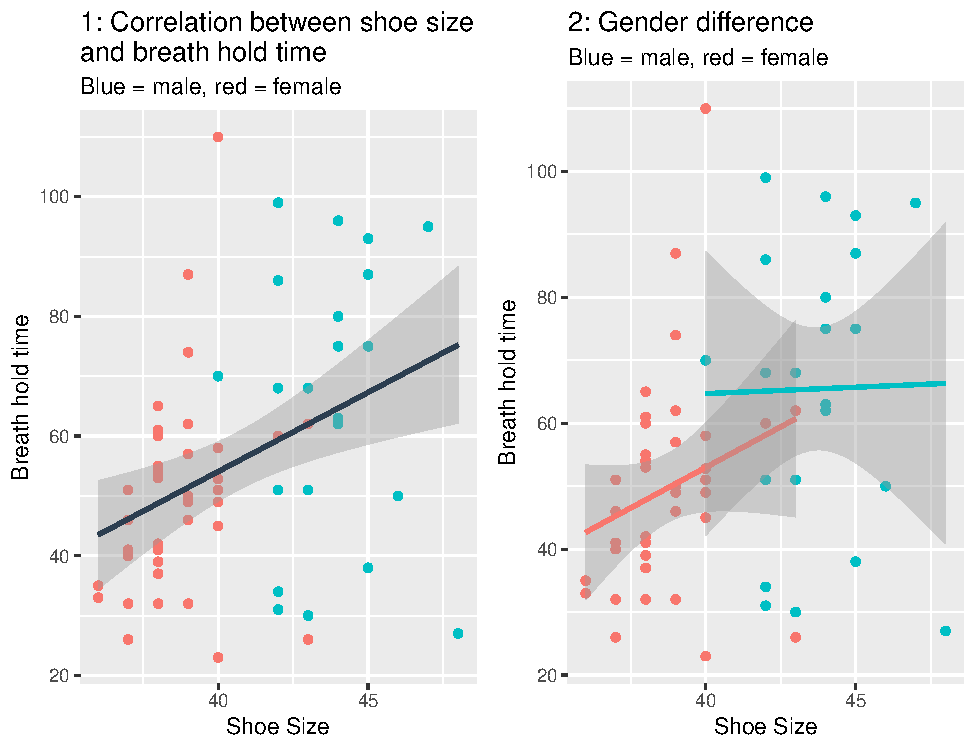
\includegraphics{Personality-Data-Analysis-Portfolio-1_files/figure-latex/unnamed-chunk-14-1.pdf}
\caption{\label{fig:unnamed-chunk-14}Correlation between shoe size and breath hold time with regression lines}
\end{figure}

The graphs show a correlation between shoe size and ability to hold breath but we can't talk about a difinite correlation between the two variables. On the differences between genders, females generally have a lower ability to hold their breath compared to males when looking at the graph's scatterplot and if we calculate the means: \$mean\_f=\$49.6528947 and \$mean\_m=\$65.4583333, we can see that the likely reason for the linear regression's slope in visualization 1 is this difference in mean and in shoe size between genders.

The reason we can see this is that visualization 2 shows us that there is no apparent correlation between shoe size and breath\_hold in the male regression. Additionally the error visualization in the graphing of the linear regression shows us that the variance is too large to conclude direct correlation.

But beyond just looking at the graphs, we can analyze the correlation between the two variables and see if it's statistically significant. By setting up a correlation matrix, we can see if there's any good correlation between the values. balloon, sound\_level\_pref, hours\_music\_per\_week and tongue\_twist have also been added because it would be interesting to see if there's a correlation between any of these in addition to the other two.

This is done by melting a data frame with the variable correlations into a three-variable data frame and inputting it in the geom\_tile() function that creates color tiles based on correlation (0:1).

\begin{Shaded}
\begin{Highlighting}[]
\KeywordTok{p_load}\NormalTok{(reshape2)}
\NormalTok{cormat <-}\StringTok{ }\NormalTok{df[, }\KeywordTok{c}\NormalTok{(}\StringTok{"hours_music_per_week"}\NormalTok{, }\StringTok{"sound_level_pref"}\NormalTok{, }\StringTok{"shoesize"}\NormalTok{, }\StringTok{"breath_hold"}\NormalTok{, }
    \StringTok{"balloon"}\NormalTok{, }\StringTok{"tongue_twist"}\NormalTok{)]}
\NormalTok{cormat <-}\StringTok{ }\KeywordTok{round}\NormalTok{(}\KeywordTok{cor}\NormalTok{(cormat), }\DecValTok{2}\NormalTok{)}
\NormalTok{melted_cormat <-}\StringTok{ }\KeywordTok{melt}\NormalTok{(cormat)}

\KeywordTok{ggplot}\NormalTok{(melted_cormat, }\KeywordTok{aes}\NormalTok{(Var1, Var2, }\DataTypeTok{fill =}\NormalTok{ value)) }\OperatorTok{+}\StringTok{ }\KeywordTok{geom_tile}\NormalTok{()}
\end{Highlighting}
\end{Shaded}

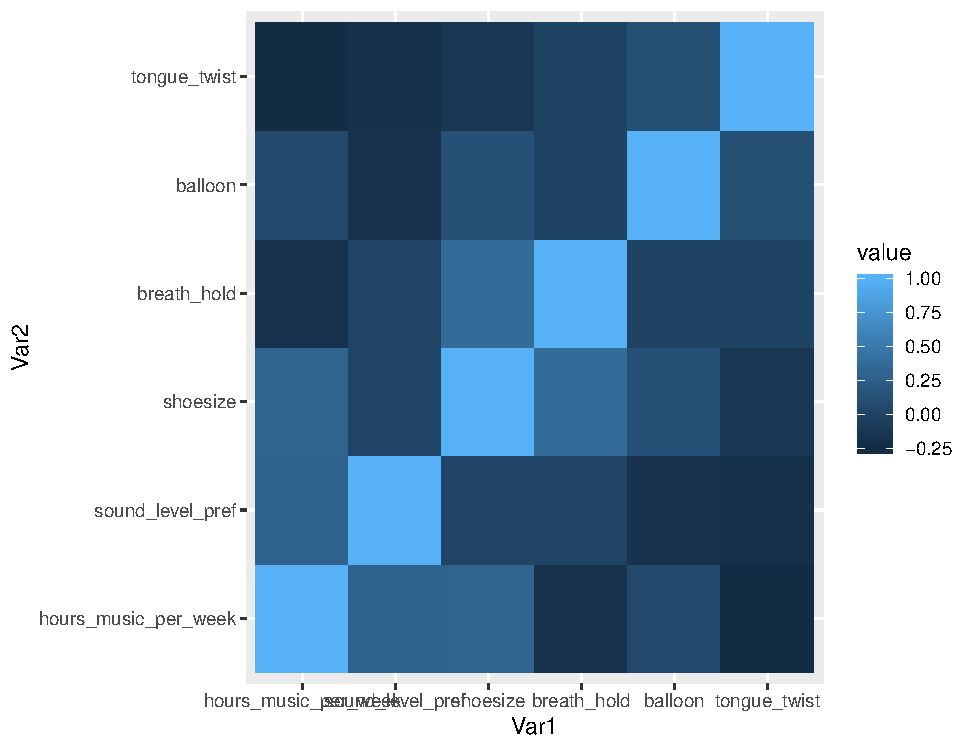
\includegraphics{Personality-Data-Analysis-Portfolio-1_files/figure-latex/unnamed-chunk-15-1.pdf}
Interestingly, we see a small correlation between hours\_music\_per\_week and sound\_level\_pref as well as shoesize and hours\_music\_per\_week. These are definitely not statistically significant (\(\rho=cor(hours, sound\_level)=\) 0.2848) but a hypothesis could have been that the hours of music correlates to preference for louder environments though this has just been disproven in our sample.

Besides being able to see the correlations of these variables on the geom\_tile, to analyze the correlation between shoesize and breath\_hold, we will calculate this correlation using the cor() function:

\(\rho = cor(shoesize, breath\_hold)=\) 0.3826

As it equals 0.38, there is no significant correlation (\(\rho>0.95\)). We can thereby conclude that there's no significant relation between shoesize and breath\_hold but that the gender influences the statistical probability of having a good skill in holding one's breath.

\hypertarget{appendix}{%
\section{Appendix}\label{appendix}}

1: Improved readability prototype

\begin{figure}
\centering
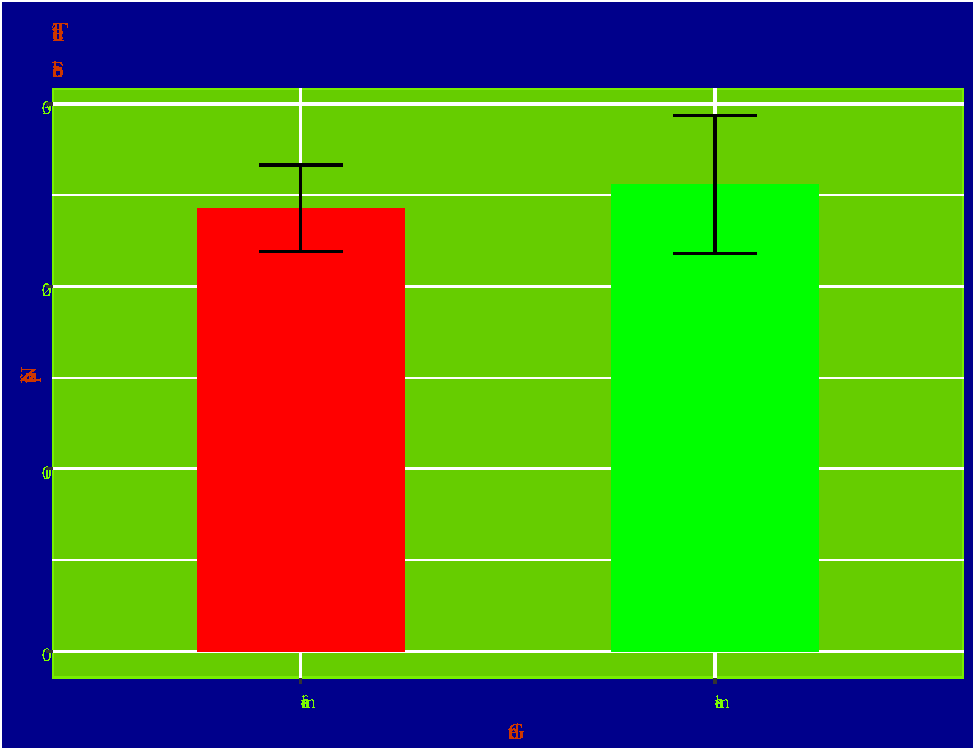
\includegraphics{Personality-Data-Analysis-Portfolio-1_files/figure-latex/unnamed-chunk-17-1.pdf}
\caption{\label{fig:unnamed-chunk-17}Improved readability prototype}
\end{figure}

\begin{verbatim}
> [1] "nice"
\end{verbatim}

\hypertarget{references}{%
\section*{References}\label{references}}
\addcontentsline{toc}{section}{References}

\hypertarget{refs}{}
\leavevmode\hypertarget{ref-eser_association_2008}{}%
Eser, Ilker, Frank Schwendeman, Daniel S. Durrie, and Jason E. Stahl. 2008. ``Association Between Ocular Dominance and Refraction.'' \emph{Journal of Refractive Surgery} 24 (7): 685--89. \url{https://doi.org/10.3928/1081597X-20080901-07}.


\end{document}
